\chapter{Supposing} \label{supp}

Our objective is to figure out the difference between valid and
invalid arguments.  We will break this objective down into two
sub-objectives.  First, we will try to write down enough rules so that
we could reproduce any valid argument by chaining those rules
together.  Second, we will {\it not} write down a rule that could
actually lead to our producing an invalid argument.

We will say that a system of logic is \emph{complete} just in case it
has enough rules to reproduce all the intuitively valid
arguments.\footnote{At this stage, we'll have to content ourselves
  with the vague notion of ``intuitively valid.''  We'll investigate a
  more precise notion -- of truth-preservation -- in Chapter
  \ref{meta}.}  It would be completely easy to produce a complete
system of logic, if we didn't have any further objective.  For
example, if you said that ``every inference is permitted,'' then you'd
automatically be able to reproduce any valid argument.  Obviously,
that would be a foolish way of proceeding.  But there's also danger in
the opposite direction.  If we write down too few rules, then there
may be some valid argument that our system cannot reproduce.  And what
a shame that would be if we put on a pair of logical glasses, so to
speak, that prevented us from seeing some valid arguments.  The
consequence of doing that is that we might fail to recognize some
important truths, even truths that could change our lives.

In the previous chapter we wrote down a few rules of inference that we
took to be obviously valid.  Now the question that faces us is whether
we wrote down enough rules.  In other words, just using the rules from
the previous chapter, can we reproduce every valid argument?

That's not such an easy question to answer.  Consider the following
argument:
\[ \begin{array}{l >{$}p{2cm}<{$} p{1.5cm}}
     (1) & P\vee Q & A \\
     (2) & \neg P & A \\
     (3) & Q & 1,2 \; ?\end{array}
\]
Now, this argument seems obviously valid to me.\footnote{Most
  logicians in history shared this opinion.  So much so that they
  invented a name for this apparently valid argument: \emph{modus
    tollendo ponens}, nowadays usually called \emph{disjunctive
    syllogism}.  But note well: disjunctive syllogism is {\it not} a
  basic inference rule of our system.}  If you know that one of two
things is true, either $P$ or $Q$, and if you know that $P$ is not
true, then surely you know that $Q$ is true.  But can we prove this
argument using the rules from the previous chapter?  The answer, in
short, is no: we cannot prove this argument using the rules from the
previous chapter.  One hint is that this argument uses a disjunctive
premise --- i.e.\ a premise with $\vee$ --- and we don't yet have any
rule that takes a disjunctive sentence as its input.

(Aside for the ambitious student: you can actually {\it prove} that
the argument above cannot be derived from the rules laid down in the
previous chapter.  In particular, let's suppose that $P\vee Q$ is
always true, no matter whether $P$ and $Q$ are true.  It's easy to see
then that the rules from the previous chapter would always take true
sentences to true sentences.  However, the argument above could derive
a false sentence from two true sentences.)

So, the sequent $P\vee Q,\neg P\vdash Q$ is intuitively valid, but it
is not provable from the rules given in the previous chapter.  Since
our objective is to be able to reproduce all intuitively valid
arguments, we need to add some more rules so that we can derive this
argument.  One thing we could do is whenever we find a new argument
that is intuitively valid, we could just add this argument itself as a
new rule to our system.  However, that would be shortsighted: our
system of rules would grow to unwieldy proportions.  What's more, the
result wouldn't really be a {\it system}, because a system should have
some rhyme and reason.  We don't want to pick our basic logical rules
randomly.  We want to pick them on the basis of some principle.  The
operative principle from Chapter \ref{deduce} is that each special
logical word (and, or, if-then, not) corresponds to certain inferences
that we are permitted to make.  For example, a conjunction $P\wedge Q$
licenses the inference to $P$ and $Q$ individually.

Now, we have an elimination rule for $\to$, but no corresponding
introduction rule.  And we have an introduction rule for $\vee$, but
no corresponding elimination rule.  So, it would make sense to expand
our system by adding the corresponding rules.  Let's begin with the
idea of arguing for a conditional statement.

Suppose that you want to convince somebody that \textit{if $\phi$ then
  $\psi$}, where $\phi$ and $\psi$ are some sentences that are either true or
false (but you might not know which).  For example, you might want to
convince somebody that if corporate taxes are reduced, then the budget
will not be balanced.  Or you might want to convince somebody that if
God doesn't exist, then there are no moral rules.  Or you might want
to convince somebody that if $m$ is an rational number, then $m^2$ is
a rational number.  In many such cases, the argument for \textit{if
  $\phi$ then $\psi$} begins with a curious maneuver: the arguer says
\textit{suppose that $\phi$}.  For example, if I wanted to convince you
about $m^2$ being a rational number, I might say:
\begin{quote} \underline{Suppose} that $m$ is a rational number.  In
  that case, $m=a/b$ for two integers, and $m^2=a^2/b^2$, which means
  that $m^2$ is also rational.  \end{quote} Then I would conclude by
saying {\it therefore, if $m$ is rational, $m^2$ is also rational}.

The word ``suppose'' plays a very special role here, and one that
might not seem logical at all.  You might have thought that being
logical boils down to correctly inferring things from a collection of
already established facts.  However, that is most definitely {\it not}
what is happening in the ``suppose'' maneuver.  When a person says
``suppose'', she is not deducing anything.  Quite to the contrary, she
is asking her interlocutor to play a sort of game with her.  In fact,
she is asking her interlocutor to accept something temporarily that
they don't know to be true.

Now, you might think that allowing suppositions is a recipe for
logical disaster.  If people can just suppose whatever they want, then
how is that logical?  Well, it becomes logical when the two
discussants keep track of which suppositions they have made.

Imagine then, as an idealized account of what actually occurs in
argumentation, that when we sit down to argue, we set out a scorecard.
At the beginning of our argument, our scorecard contains a list of
agreed-upon premises for our discussion.  For example, the two of us
might agree to use the word ``rational'' for numbers of the form
$a/b$, and we might agree that $(a/b)^2=a^2/b^2$, etc.  During our
subsequent argumentation, each of us is allowed to cite any one of
these agreed upon premises.  However, besides citing agreed upon
premises, each of us is permitted to ``suppose'' that something is
true --- provided that we mark down clearly on the score card that
we've added a new supposition.  Once we've added this new supposition,
we can continue drawing inferences; however, it would be a terrible
logical mistake to think that the conclusions we derive follow from
the {\it original} list of premises.  No, the conclusions we now
derive depend on the original list of premises, plus the additional
supposition.

So far so good.  However, what if we want to see what follows from the
original list of premises?  Is there a way to go about ``unsupposing''
things that we supposed during the course of an argument?  It's here
where a $\to$ introduction rule could come in handy, because a
conditional conclusion is just that: it's {\it conditional} on
something.  In particular, if you suppose that $\phi$, and then you
--- perhaps undertaking a long detailed argument --- derive $\psi$,
then you are entitled both to conclude that $\phi\to \psi$, and to
forget that you supposed $\phi$ in the first place.  For, when you say
that $\phi\to \psi$, you are now explicitly noting that the conclusion
($\psi$) depends on a supposition of $\phi$.

This then is the idea behind the $\to$ introduction rule.
Fortunately, the implementation of this idea is quite simple.  The
first thing we need to do is to introduce the ``score card'' to keep
track of the suppositions in an argument.  We will do so by adding a
new column to the left of the line numbers in a proof.  This new
column will give a running tabulation of the suppositions in force at
each stage of the argument.  So, now if I ask you to prove something,
say $P\vdash P\vee Q$, then the score card begins with agreed-upon
premise $P$.  This premise is the supposition that we make together,
at the very beginning of the argument.  Accordingly, the first line of
your proof would read:
\[ \begin{array}{l l
      >{$}p{1cm}<{$} p{1.5cm} l } 1 & (1) & P & A \end{array} \] This
line has four columns, one of which is new.  The leftmost column
contains the number ``$1$'', which we call the \gls{dependency
  number}, and it serves as the ``score card'' of the argument.  In
other words, the leftmost column tells you which suppositions are in
force at that stage of the argument. \index{dependency number}

So, we are proposing an update in the way we think of proofs.  A proof
is not a list of sentences, where each sentence is deduced from
previous sentences in the list.  Instead, a proof is a list of
\glspl{sequent}, where each sequent amounts to a statement that some
list of sentences implies some other sentence.  Correspondingly, the
inference rules should be reconceived as telling us which new sequents
can be generated from sequents that we have already obtained.

This new way of thinking about proofs is more democratic than the old
way from the last chapter.  In the last chapter, all proofs began with
given premises.  From now on, anyone can add new assumptions at any
stage of a proof.  That is, for any sentence $\phi$, you are permitted
to write
\[ \begin{array}{l l
      >{$}p{1cm}<{$} p{1.5cm} l } n & (n) & \phi & A \end{array} \]
which expresses the sequent $\phi\vdash\phi$, since the dependency
number ``$n$'' points to the sentence $\phi$.  The official rule for
making assumptions is the following: \bigskip
\begin{tcolorbox}[enhanced,width=9.7cm,title=rule of assumptions (A),attach boxed title to top
  left={yshift=-2mm,xshift=4mm},boxed title style={sharp corners}] 
At any stage in an argument, you are permitted to suppose anything you want to, as long as you add
  that supposition to the argument's score-card.  
\end{tcolorbox} \bigskip
Here the schematic statement of the rule of assumptions is the strange
looking:
\[ \begin{array}{c c}
       \mbox{} \\ \hline
     \phi\:\vdash\: \phi \end{array} \]
The horizontal line indicates that one is permitted to infer what lies
below the line if one already has what lies above the line.  In this
case, nothing lies above the line, which means that one is permitted
to infer $\phi\vdash\phi$ in any situation.

The above proof might then continue as follows:
\[ \begin{array}{l l
     >{$}p{2cm}<{$} p{1.5cm}}
     1 & (1) & P  & A \\ 
     1 & (2) & P\vee Q & 1 $\vee$I \end{array} \] Here the far right column is the same as
the previous chapter: it says that line $2$ is justified by
application of $\vee I$ to line $1$.  The far left column has the
number ``$1$'' to indicate the the supposition at line $1$ is still in
force at line $2$.  In general, for each of the rules that you learned
in the previous chapter, the suppositions in force when the premises
were asserted will still be in force when the conclusion is asserted.
For example, the conjunction introduction rule should be reformulated as
saying:
\begin{quote} Given sequents $\Gamma\vdash\phi$ and
  $\Delta\vdash\psi$, one may derive the sequent $\Delta
  ,\Gamma\vdash\phi\wedge\psi$. \end{quote} Or, written out graphically, $\wedge$ intro
appears as follows:
\[ \begin{array}{l l >{$}p{1.5cm}<{$} l}
  \Gamma & (\ast ) & \phi   \\
  \Delta & (\star ) & \psi \\
  \Gamma ,\Delta & (\dagger ) & \phi \wedge \psi & \ast ,\star
                                                 \wedge\mathrm{I}   
   \end{array} \]
In other words, when we use conjunction introduction on lines $\ast$
and $\star$ to derive line $\dagger$, the dependencies of line
$\dagger$ should be the union of the dependencies of lines $\ast$ and
$\star$.

Let's see this use of suppositions in action in the proof of the
sequent $(P\vee Q)\to R,P\vdash R$.  Here we are asked to prove $R$
under the suppositions $(P\vee Q)\to R$ and $P$.  We begin then by
writing down those suppositions, giving a new number for each in the
left-hand column.
\[ \begin{array}{l l >{$}p{2.5cm}<{$} p{1.5cm}}
  1 & (1) & (P\vee Q)\to R &  A \\
  2 & (2) & P & A \\
  2 & (3) & P\vee Q & 2 $\vee$I \\
  1,2 & (4) & R  & 1,3 MP \end{array} \]
We then proceed as we did in the previous chapter.  First we derive
line $3$ from line $2$ using the $\vee$I rule; and we accordingly
carry the supposition from line $2$ down to line $3$.  Then we derive
line $4$ from lines $1$ and $3$ using the MP rule; and we accordingly
carry the suppositions from line $1$ and $3$ down to line $4$.

It would be a good idea now to go back and do a few of the proofs from
the previous chapter, but now keeping explicit track of the
suppositions in force at each stage.  The process may be a bit
tedious, but it will be conceptually simple, because whenever you
apply a rule, you simply have to copy the suppositions from the lines
you cite onto the new line.  For example:
\[ \begin{array}{l l >{$}p{3cm}<{$} p{2cm}}
     1 & (1) & P & A \\
     2 & (2) & Q & A \\
     1,2 & (3) & P\wedge Q & 1,2 $\wedge$I \\
 1,2 & (4) & (P\wedge Q)\wedge P & 3,1 $\wedge$I  \end{array} \]
In this example you can see that the list of suppositions doesn't need
to contain duplicate numbers.  To derive line $3$, we cited lines $1$
and $2$, and so line $3$ depends on whatever lines $1$ and $2$
depended on.  To derive line $4$, we cited lines $3$, and $1$, and
so line $4$ depends on whatever those lines depended on.  However, we don't write ``$1,1$'' in the left-hand
column, because it's enough to note that the assumption of $1$ is in force.
Similarly, it doesn't matter in what order dependency numbers occur.  For
example, having $1,2$ in the left-hand column is the same as having
$2,1$.

Similarly, consider the following proof that uses the other rules from
last chapter.
\[ \begin{array}{l l >{$}p{3cm}<{$} p{2cm}}
     1 & (1) & P\wedge \neg\neg Q & A \\
     1 & (2) & \neg\neg Q & 1 $\wedge$E \\
     1 & (3) & Q          & 2 DN \\
     1 & (4) & Q\vee R    & 3 $\vee$I \end{array} \]
The use of conjunction elimination on line $2$ cites line $1$, and
so we copy the dependencies of line $1$ to line $2$.  The same goes
for the use of DN on line 3, and the use of disjunction introduction
on line 4. 

Now we can come back to the $\to$ introduction rule.  The whole point
of keeping track of suppositions is so that {\it you}, the reasoner,
can strategically make new suppositions, and then later discharge
these assumptions.  Hence, the $\to$ introduction rule, which is also
called \emph{conditional proof (CP)}, should look like this:
\begin{quote} If, within context $\Gamma$, you suppose that $\phi$,
  and if from $\Gamma$ and $\phi$ you derive $\psi$, then you may
  assert, in the same context $\Gamma$, the conditional
  $\phi\to \psi$.  \end{quote} Now we have to see how to implement
this general idea concretely in terms of line numbers of a proof.
Let's say that you suppose $\phi$ on some specific line $m$ of your
proof:
\[ \begin{array}{>{$}p{2cm}<{$} l >{$}p{1.5cm}<{$} p{2cm}}
     \qquad\qquad m & (m) & \phi & A  \end{array} \]
Notice that the dependency number $m$ is the same as the line number,
which will always be the case for a supposition (i.e.\ assumption).
Now suppose that you have another line like this:
\[ \begin{array}{l l >{$}p{1.5cm}<{$} p{2cm}}
    n_1,\dots ,n_k,m & (n) & \psi \end{array} \] The conditional proof
rule says that from these two lines, you may infer the line
\[ \begin{array}{l l
      >{$}p{1.5cm}<{$} p{2cm}} \quad n_1,\dots ,n_k & (n') & \phi\to \psi &
    $m,n$ CP \end{array} \] Notice how the dependency on $m$ is
dropped in the move from line $n$ to line $n'$.  Dropping the
dependency signals that we are no longer supposing that $\phi$; we are
now asserting that {\it if} $\phi$ then $\psi$.

Here's a simple example of the kind of move permitted by conditional
proof.  The MT rule says $\neg P$ can be inferred from $P\to Q$ and
$\neg Q$.  Now, imagine that everyone agrees that $P\to Q$, but that
not everybody agrees that $\neg Q$.  Nonetheless, you should be able
to convince all logical people that {\it if} $\neg Q$ then $\neg P$.
Your argument could be formalized as follows:\marginnote{contrapositive
  \\ $P\to Q\:\vdash\:\neg Q\to\neg P$}
\[ \begin{array}{l l >{$}p{2.5cm}<{$} p{2cm}}
     1 & (1) & P\to Q & A \\
     2 & (2) & \neg Q & A \\
     1,2 & (3) & \neg P & 1,2 MT \\
     1 & (4) & \neg Q\to\neg P & 2,3 CP \end{array} \]
Our formal system doesn't pick up the nuance that everyone agrees (in
this example) to the first assumption (line 1), whereas you made the
second assumption (line 2) for the sake of argument.  But no matter
--- the point is just that now we can model this ubiquitous practice
of supposing things for the sake of argument.

\bigskip 
\begin{tcolorbox}[enhanced,width=10cm,title=conditional proof (CP),attach boxed title to top
  left={yshift=-2mm,xshift=4mm},boxed title style={sharp corners}] 
A proof of $\psi$ from dependencies $\Gamma ,\phi$ may be converted to a
proof of $\phi\to \psi$ from dependencies $\Gamma$.  \newline Schematically: 
  $\begin{array}{r@{\;}c@{\;}l}
       \Gamma ,\phi & \vdash & \psi \\ \hline
       \Gamma & \vdash & \phi\to \psi \end{array}$
\end{tcolorbox} \bigskip

Don't try to memorize the CP rule by staring at it.  Instead: watch it
being used, and use it yourself.  Let's begin with a proof that
conditionals are transitive, i.e.\ that if $P\to Q$ and $Q\to R$ then
$P\to R$.
\[ \begin{array}{l l >{$}p{2.5cm}<{$} p{2cm}}
  1 & (1) & P\to Q & A \\
  2 & (2) & Q\to R & A \\
  3 & (3) & P & A \\
  1,3 & (4) & Q & 1,3 MP \\
  1,2,3 & (5) & R & 2,4 MP \\
  1,2 & (6) & P\to R & 3,5 CP \end{array} \]
The assumption on line 3 is motivated by the idea that we want to
prove $P\to R$.  So, when we assumed $P$ on line 3, we did so
thinking, ``all we have to do is derive $R$, and then we can use CP to
get $P\to R$''.  Notice that as soon as we've made the assumption of
$P$, we are now back in the easy territory of the previous chapter.
Now we just deduce and deduce until we get $R$.  Then, at line 6, we
remember what we were trying to do: we ``discharge'' the assumption on
line 3 by invoking CP.

In the following proof, we go to a second hypothetical level.  That
is, we make one supposition, and prepare to deduce.  But then we see
that the conclusion we want is a conditional, so it makes sense to
make a second supposition.  
\[ \begin{array}{l l >{$}p{2.5cm}<{$} p{2cm}}
  1 & (1) & (P\wedge Q)\to R & A \\
  2 & (2) & P & A \\
  3 & (3) & Q & A \\
  2,3 & (4) & P\wedge Q & 2,3 $\wedge$I \\
  1,2,3 & (5) & R & 1,4 MP \\
  1,2 & (6) & Q\to R & 3,5 CP \\
     1   & (7) & P\to (Q\to R) & 2,6 CP \end{array} \]
On line 2, we suppose $P$, with the intention of proving $Q\to R$.
And then it's like we start all over again.  Since we want to prove
$Q\to R$, we assume $Q$.  Then we're back in the gentle territory of
the previous chapter, deducing until we get $R$ on line 5.  On line 6,
we use CP to return from the second hypothetical level to the first.
On line 7, we use CP again to return from the first hypothetical level
to the zeroth.

Things can become confusing when you try to prove a conditional whose
antecedent is a complex sentence.  For example, suppose that you want
to prove $(P\wedge Q)\to R$ from $P\to (Q\to R)$.  Here you must avoid
the temptation to assume $P$ and $Q$ on separate lines, and then use
$\wedge$ introduction.  For then you'd have two dependency numbers,
whereas CP only gets rid of one.  To use CP properly, you've got to
assume exactly the antecedent of the conditional you are trying to
prove.  Consider, for example, the following proof.
\marginnote{prefixing \\ $Q\to R\:\vdash\: (P\to Q)\to (P\to R)$}
\[ \begin{array}{l l >{$}p{4cm}<{$} p{2cm} l}
     1 & (1) & Q\to R & A \\
     2 & (2) & P\to Q & A \\
     3 & (3) & P      & A \\
     2,3 & (4) & Q    & 2,3 MP \\
     1,2,3 & (5) & R  & 1,4 MP \\
     1,2   & (6) & P\to R & 3,5 CP \\
     1 & (7) & (P\to Q)\to (P\to R) & 2,6 CP \end{array} \] Here we're
 trying to prove $(P\to Q)\to (P\to R)$, which is a conditional whose
 antecedent is a conditional.  Note well: the fact that the antecedent
 is a conditional makes no difference at all to the fact that
 \textit{you should assume the antecedent}.  You shouldn't try to
 prove $P\to Q$, and you shouldn't (yet) assume $P$, for neither of
 those would do you any good.  Instead, assume $P\to Q$, and then take
 up the next problem, i.e.\ of proving $P\to R$ from $Q\to R$ and
 $P\to Q$.

 Before we set you loose on some exercises, we'll explain a method that
 can make some difficult proofs easier.  Consider, for example, the
 sequent $\neg P\vdash \neg (P\wedge Q)$, which is sometimes called
 \textit{weakening}.  A direct attack on this sequent will only lead
 to frustration: from an assumption of $\neg P$, there is no amount of
 conjoining or disjoining that will get you to $\neg (P\wedge Q)$.  We
 recommend, then, that you prove the contrapositive, that is
 $P\wedge Q\vdash P$.  Of course, that proof is trivially easy, and
 then you can complete the proof of weakening as follows:
 \[ \begin{array}{llp{2cm}ll}
      (P\wedge Q)\to P & & CP \\
      \neg P & &  A  \\
      \neg (P\wedge Q) & & MT \end{array} \] In summary, you can use
 MT to transform a proof of a sequent into a proof of its contrapositive.

  \newcommand{\sitem}{\stepcounter{enumi}\item[\!\!$^\ast$\theenumi.]}

\begin{exercises} Prove the following sequents.
  \begin{enumerate}
  \item $P\:\vdash\: Q\to (P\wedge Q)$
  \item $(P\to Q)\wedge (P\to R)\:\vdash\: P\to (Q\wedge R)$
\item permutation: $P\to (Q\to R)\:\vdash\: Q\to (P\to R)$
\item suffixing: $P\to Q\:\vdash\: (Q\to R)\to (P\to R)$
\item contraction: $P\to (P\to Q)\:\vdash\: P\to Q$  
\item exportation: $P\to (Q\to R)\:\vdash\: (P\wedge Q)\to R$
\item strengthening: $(P\vee Q)\to R\:\vdash\: P\to R$
\item weakening: $\neg P\:\vdash\: \neg (P\wedge Q)$  
\item \gls{dm}: $\neg (P\vee Q)\:\vdash\: \neg P\wedge\neg
  Q$ \newline (Hint: prove the individual conjuncts, then use $\wedge$
  introduction.)
%% use contrapositive to get $\neg (P\vee Q)\vdash \neg P$  
%% not $P\to R\:\vdash\: (P\vee Q)\to R$
\sitem $P\to \neg P\:\vdash\:\neg P$  
  \end{enumerate}
\end{exercises}


\section{Proofs without dependencies}

Now that you have a rule for discharging assumptions (viz.\
conditional proof), you can produce valid arguments that end without
{\it any} assumptions in force.  For example, here's a proof of the
trivial truth: if $P$ then $P$.
\[ \begin{array}{l l >{$}p{1.5cm}<{$} p{1.5cm}}
  1 & (1) & P & A \\
    & (2) & P\to P & 1,1 CP
   \end{array} \]
We write this sequent as $\vdash P\to P$, with no premises on the
left-hand side of the turnstile; and in this case, we say that $P\to P$
is \emph{provable}.  The result then is a statement that
anybody is permitted to assert in any circumstance whatsoever.  

Before we set you loose proving things, we need to warn you of one
danger: conditional proof must only be used when the first of the two
lines is an assumption.  If you don't observe that restriction, then
you could prove too much, as in the following argument.
\[ \begin{array}{l l >{$}p{2cm}<{$} p{1.5cm} p{3cm}}
     1 & (1) & P\wedge Q  & A \\
     1 & (2) & P  & 1 $\wedge$E \\
     1 & (3) & Q &  1 $\wedge$E \\
       & (4) & P\to Q & 2,3 CP &
                                 $\Longleftarrow$
                                 incorrect \end{array} \] Here we
tried to use CP with lines $2$ and $3$, even though line $2$ was not an assumption.  But line $2$ depends on $P\wedge Q$, which is logically stronger than $P$, and it's not justified to erase the dependency on $P\wedge Q$ when conditionalizing only on $P$.

\begin{exercises} Prove the following sequents.
  \begin{enumerate}
  \item $\vdash\:(P\wedge Q)\to (Q\wedge P)$  
  \item $\vdash\:(P\wedge Q)\to P$  
  \item $\vdash\:Q\to (P\to Q)$
  \item $\vdash\:Q\to (P\to P)$
  \sitem \gls{em}: $\vdash \:P\vee \neg P$
%% prove \neg (P\vee \neg P)\vdash P\wedge \neg P; use CP and MT
  \end{enumerate}
\end{exercises}




%% I think it's possible now to prove $(\neg P \to P)\to P$


\section{Paradoxes of material implication} 

Before we move on to our last two inference rules, we should talk a
little bit about something disconcerting that can happen with
conditional proof.  It will be simplest just to write down two (valid)
proofs.  If these proofs don't bother you, then there's really no need
to read the rest of this section!

We first prove a result known as \emph{positive paradox}: from the
assumption that $Q$, it follows that $P\to Q$.  Since logic is
completely general, this result implies for example, that from the
assumption that this match will light when struck, it follows that if
we are under water, then this match will light when struck. \marginnote{positive paradox \\ $Q\:\vdash\: P\to Q$} 
\[ \begin{array}{l l >{$}p{2cm}<{$} l}
  1 & (1) & Q & \mathrm{A} \\
  2 & (2) & P & \mathrm{A} \\
     1 & (3) & P\to Q & 2,1 \;\mathrm{CP} \end{array} \]

Here the new supposition $P$ occurs on line 2, after the conclusion
$Q$ had already been asserted.  This maneuver might seem like an
egregious abuse of the rule CP, which was intended to capture the idea
of making a new supposition in order to derive a certain conclusion.
In this proof, the conclusion was already there, and the new
supposition wasn't needed to get it.  So isn't it quite misleading to
conclude that {\it if $P$ then $Q$}?  After all, $Q$ had already been
supposed before $P$ was supposed.

If you're a bit unhappy that this proof counts as valid, then you are
in good company.  Ever since the early days of modern symbolic logic,
back in the early 1900s, philosophers have wondered whether something
has gone wrong.  We can't go deeply into that debate here, but it's
worthwhile seeing that it's not so easy to fix the CP rule to prevent
this kind of argument.  The most obvious proposal to fix the CP rule
is to require that the antecedent (in this case $P$) is actually used
to derive the consequent.  We could try to enforce this requirement by
saying that the line on which the consequent occurs must depend on the
line on which the antecedent is assumed.  The proof above would
violate this revised rule, because 2 does not appear among the
dependencies on line 1.

Unfortunately, when this revised rule is brought into interaction with
the other rules, it proves to be just as liberal as the original rule.
Consider the following proof that uses the more conservative rule.
\[ \begin{array}{l l >{$}p{2cm}<{$} p{2cm}}
     1 & (1) & Q & A \\
     2 & (2) & P & A \\
     1,2 & (3) & P\wedge Q & 1,2 $\wedge$I \\
     1,2 & (4) & Q & 3 $\wedge$E \\
     1 & (5) & P\to Q & 2,4 CP \end{array} \] Here CP is applied to
lines 2 and 4, and the supposition made on line 2 is used to get line 4.  So, this proof obeys the revised rule, despite the fact that it allows us to derive exactly the same conclusion as the previous proof.  In fact, it's not too hard to see that anything that can be derived with the original ``liberal CP rule'' can be derived with the new ``conservative CP rule''.  So, the new rule is only apparently more conservative than the old, and we might as well allow ourselves to use the old one.


There's another pair of results that are perhaps even more troubling
than positive paradox.  We'll now write one proof that proves a couple
of different paradoxical sequents.   
\[ \begin{array}{l l >{$}p{2cm}<{$} p{2cm}}
     1 & (1) & \neg P      & A       \\
     2 & (2) & P           & A        \\
     3 & (3) & \neg Q      & A        \\
     2 & (4) & \neg Q\to P & 3,2 CP   \\
     1,2  & (5) & \neg \neg Q & 4,1 MT  \\
     1,2  & (6) & Q           & 5 DN     \\
     1 & (7) & P\to Q & 2,6 CP \end{array} \] The sixth line of
 the proof demonstrates \gls{efq}, which translated loosely means, ``from the false, everything follows''.\marginnote{ex falso quodlibet \\
   $\neg P,P\:\vdash\: Q$} This sequent is also sometimes called
 \emph{explosion}, because it shows that $P$ and $\neg P$ together
 form a ticking time-bomb that, when triggered, ejects all other
 sentences.  The last line proves \emph{negative paradox}, which shows
 that a conditional follows from the negation of its
 antecedent.\marginnote{negative paradox \\ $\neg P\:\vdash\: P\to Q$}

 \gls{efq} has bothered logic students like yourself for well over a
 thousand years.  It seems exactly wrong, you might think, that a
 person with inconsistent beliefs (such as $P$ and $\neg P$) has
 ``inferential omnipotence'', i.e.\ they can infer any sentence $Q$
 whatsoever.  But that worry stems from an ambiguity in the English
 verb ``to infer that''.  For example, if you overheard me say that
 ``I infer that the sun will collapse,'' you might assume that I
 believe that the sun will collapse.  However, there is a weaker sense
 of ``infer'' in which it simply means that a person reasons from some
 claims (which that person need not believe) to other claims (which
 that person need not believe).  For example, I might have inferred
 that the sun will collapse from a contrary-to-fact supposition about
 the mass of the sun.  I might not actually believe that the mass of
 the sun is so large, but I nonetheless believe that if its mass were
 so large, then it would collapse.
 
 So, we should keep it clearly in mind that the typical use of logical
 reasoning is not to start from a set of premises about which we are
 completely certain, and then to reason to additional conclusions.
 Much more typically, logic is used to reason from premises that we do
 not necessarily believe to a conclusion that we don't necessarily
 believe.  In logic it's not the conclusions that we're interested in,
 but in the connection between premises and conclusions.  And logic
 doesn't have anything to say about whether one should accept the
 conclusions of valid arguments from the premises that one already
 accepts.  Indeed, what logic might be telling you is that you ought
 to reject one of the premises.  That's certainly what I would
 recommend doing if you found yourself with premises that imply both
 $P$ and $\neg P$.

\section{Reasoning from disjunctive premises}

Imagine that you're stuck in a dark room, and that you cannot see
outside.  However, you have a phone, and you can get text messages
from your friend, Angelina, who is outside.  But Angelina loves to be a
bit elusive.  If you ask her a question, she tends to reply by
asserting a disjunction.  For example, if you say, ``What's the
weather like today?'' then Angelina might say something like, ``Either
it's raining or it's snowing.''

Now, Angelina isn't completely useless to you, because you can deduce
some helpful information from the things she says.  (I'm supposing
here that Angelina always tells the truth.)  For example, suppose that
you're a member of the quidditch club; and the club has a rule that
practice is canceled on any day that it rains or snows.  In this
case, Angelina's statement ``Either it's raining or it's snowing'' is
sufficient for you to deduce that there won't be quidditch practice
today.

The inference you make is roughly the following:
\begin{quote}
  Either it's raining or it's snowing. (From Angelina) \\
  If it's raining, then there is no quidditch practice. (Club rule) \\
  If it's snowing, then there is no quidditch practice. (Club rule) \\
  Therefore, there is no quidditch practice. \end{quote}
And the form of this inference is:
\[ \begin{array}{c} P_1\vee P_2 \quad P_1\to Q \quad P_2\to Q \\
     \hline Q \end{array} \] This argument form seems obviously
to be valid, and hence we will take it as the paradigm case of how to
deduce something from a disjunctive premise.

Before proceeding to formalize the rule of disjunction elimination,
let's generalize the idea that it needs two conditional premises such
as $P_1\to Q$ and $P_2\to Q$.  Let's consider, instead, the
possibility that the conclusion $Q$ is based on two {\it reasoning
  processes}.  In this case, you know that either it's raining or it's
snowing because Angelina told you that.  Now you reason as follows:
First, {\it if} it's raining, {\it then} there is no quidditch
practice.  (Here you rely possibly on some background information
$\Delta _1$, and your reasoning process might be quite long and
intricate.)  Second, {\it if} its snowing, {\it then} there is no
quidditch practice.  (Here you might rely on some other background
information $\Delta _2$, and you might engage in another reasoning
process to arrive at $Q$.)  From your knowledge that either $P_1$ or
$P_2$ is true, and from your rigorous reasoning on a case by case
basis, you conclude with confidence that $Q$.  Of course, if you want
to produce a valid argument, then you need to keep track of all of the
background information you drew upon when reasoning about the two
cases.  That is, you may assert that $Q$ follows from the disjunction
$P_1\vee P_2$, plus the background information contained in
$\Delta _1$ and $\Delta _2$.

The overall argument can be represented visually as follows.
\begin{figure}[h]
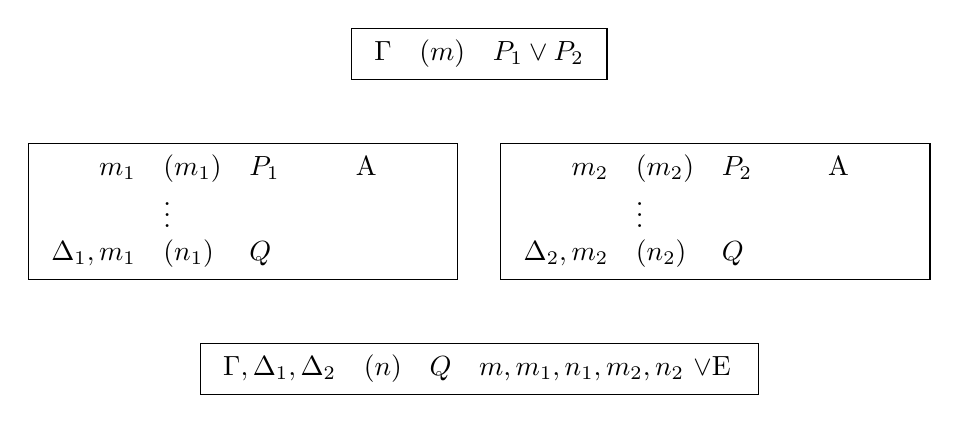
\begin{tikzpicture}  
  \node at (3,2)  (A) [draw,rectangle]{$ \begin{array}{l l l p{1cm}}
                                           \Gamma  & (m) & P_1\vee
                                                    P_2 \end{array}
                                                  $}; 
\node at (0,0) (B) [draw,rectangle]{%
  $ \begin{array}{r l >{$}p{1cm}<{$} p{1cm}}
      m_1 & (m_1) & P_1 & A \\
          & \vdots & \\
      \Delta _1,m_1 & (n_1) & Q & \end{array}$ };
\node at (6,0) (C) [draw,rectangle]{%
  $ \begin{array}{r l >{$}p{1cm}<{$} p{1cm}}
      m_2 & (m_2) & P_2 & A \\
          & \vdots & \\
      \Delta _2,m_2 & (n_2) & Q & \end{array}$ };
\node at (3,-2) (D) [draw,rectangle]{%
  $ \begin{array}{r l l p{3.25cm}}
       \Gamma ,\Delta _1,\Delta _2 & (n) & Q & $m,m_1,n_1,m_2,n_2$
                                               $\vee$E \end{array} $ % 
};
\end{tikzpicture}                                               
\caption{Disjunction elimination allows you to derive a conclusion
  from a disjunction by using two sub-arguments, one based on each disjunct.}
                                  \label{dilemma}
\end{figure}
Here we've used $\Gamma$ to represent the original background
information from which you derived the disjunction $P_1\vee P_2$.
When the $\vee$ elimination rule is invoked on line $n$, we have to
acknowledge dependency not only on $\Gamma$, but also on the
information in $\Delta _1$ and $\Delta _2$ that might have been used
in the two sub-arguments.

The reason we might need to bring other information into the
subarguments is so that we can use disjunctions together with other
premises in order to derive conclusions.  For example, consider the
premises $P\vee Q$ and $Q\to P$.  Obviously, these two premises
together should imply $P$.  Just consider the two cases: if $P$ then
of course $P$.  In the case of $Q$, we also have $Q\to P$, and hence
$P$.  But in making the second move here, we cannot forget the source
of our knowledge of $Q\to P$.  In other words, that premise needs to
be cited as well.  In official, regimented format, the argument would
go like this:
\[ \begin{array}{l l >{$}p{3cm}<{$} p{2cm}}
    1 & (1) & P\vee Q & A \\
    2 & (2) & Q\to P  & A \\
    3 & (3) & P       & A \\
    4 & (4) & Q       & A \\
    2,4 & (5) & P     & 2,4 MP \\
    1,2 & (6) & P & 1,3,3,4,5
    $\vee$E \end{array} \] The only mystery here is the exact recipe
used to calculate the dependencies of line 6.  Of course, line 6
should depend on whatever the disjunction on line 1 depends upon.  In
this case, line 1 depends only on itself.  Then we need to look at the
two sub-arguments.  The first sub-argument is completely trivial: it
starts with the assumption of $P$ on line 3, and it ends there.  It
simply infers $P$ from itself.  The second sub-argument starts with
the assumption of $Q$ on line 4; but then it uses line 2 to get line
5.  Thus, the second sub-argument presupposes line 2, and hence
whatever line 2 depends upon.  That's why we need to include line 2 in
the dependencies of line 6.  But we do {\it not} need to include lines
3 or 4 in the dependencies of line 6, because those were purely
hypothetical posits, used to see what follows from the disjunction
$P\vee Q$.  When we use disjunction elimination, we ``forget'' that
those subproofs ever happened, including the assumptions with which
they began.  We only remember the fact that both subproofs led to the
same conclusion.

We still need to tell you the {\it exact} recipe for calculating the
dependencies for a line that is justified by disjunction elimination.
We'll do that twice over, first giving a schematic proof.
\[ \begin{array}{r l >{$}p{2cm}<{$} p{3.5cm}}
    \Gamma    & (m)         & P_1\vee P_2 & \\
    m_1       & (m_1)       & P_1         & A \\
    &  \vdots     & \\
    \Delta _1,m_1    & (n_1) & Q   & \\
    m_2       & (m_2) & P_2 & A  \\
    & \vdots \\
    \Delta _2,m_2  & (n_2) & Q     \\
    \Gamma ,\Delta _1,\Delta _2 & (n) & Q &
    $m,m_1,n_1,m_2,n_2$ $\vee$E \end{array} \] That is, $\vee$E cites
five lines: a disjunction (line $m$), the assumption that begins the
first sub-argument (line $m_1$), the conclusion of the first
sub-argument (line $n_1$), the assumption that begins the second
sub-argument (line $m_2$), and the conclusion of the second
sub-argument (line $n_2$).  The dependencies of line $n$ are to be the
union of the following three collections of dependencies:
\begin{enumerate}
\item The dependencies $\Gamma$ of the disjunction $P_1\vee P_2$ on
  line $m$.
\item The dependencies $\Delta _1$ of the conclusion $Q$ on line
  $n_1$, except take away $m_1$ if it happens to occur among them.
\item The dependencies $\Delta _2$ of the conclusion $Q$ on line
  $n_2$, except take away $m_2$ if it happens to occur among them.
\end{enumerate}
In most applications, you'll follow this complicated recipe
subconsciously.  However, for those of you budding logicians who long
for full rigor, the precise set-theoretic calculation of the
dependencies on line $n$ is:
\[ \Gamma \cup (\Delta _1\backslash \{ m_1\})\cup (\Delta _2\backslash
  \{ m_2\}) ,\] which is just a symbolic representation of the words
we said previously.

As we've said before, we recommend that you try to understand abstract
rules by working on specific examples.  Let's start then with a proof
that $P$ follows from the disjunction $P\vee (P\wedge Q)$.
\[ \begin{array}{l l l p{2cm}}
    1 & (1) & P\vee (P\wedge Q) & A \\
    2 & (2) & P          & A \\
    3 & (3) & P\wedge Q  & A \\
    3 & (4) & P          & 3 $\wedge$E \\
    1 & (5) & P & 1,2,2,3,4
    $\vee$E \end{array} \] Here the first disjunct $P$ is assumed on
line $2$.  Of course, it immediately follows from the assumption of
$P$ --- without drawing any further inferences --- that $P$.  For this
reason, the application of $\vee$E on line 5 cites line 2 twice: once
as an assumption of the first disjunct, and once as the conclusion
drawn from the first disjunct.  The second disjunct $P\wedge Q$ is
assumed on line 3, and the conclusion $P$ is drawn again on line 4.
Thus, the application of $\vee$E on line 5 cites lines 3 and 4.
(Exercise: Suppose that you obtained line 5 from lines 1,2,2,3,2
instead of lines 1,2,2,3,4.  What then would be the dependencies of
line 5?)

We can now give a compact schematic statement of the disjunction
elimination rule.
\bigskip \begin{tcolorbox}[enhanced,width=7cm,title=disjunction
  elimination ($\vee$E),attach boxed title to top
  left={yshift=-2mm,xshift=4mm},boxed title style={sharp corners}]
  $ \begin{array}{c c c} \Gamma\:\vdash\: \phi \vee \psi \qquad
    \Delta ,\phi\:\vdash\:\chi \qquad \Theta ,\psi\:\vdash\:\chi \\
    \hline \Gamma ,\Delta ,\Theta\:\vdash\:\chi \end{array} $
\end{tcolorbox}
\bigskip \noindent So, the $\vee$E rule says that three separate
proofs can be converted into one proof.  Of course, you're not likely
to find those three proofs lying around; you'll usually have to make
them yourself. 

For example, suppose that you want to show $P\vee Q\vdash Q\vee P$.
Then you'd want to argue that the conclusion follows from each
disjunct separately, as follows.\marginnote{commutation \\
  $P\vee Q\:\vdash\:Q\vee P$}
\[ \begin{array}{l l >{$}p{2.5cm}<{$} p{2cm}}
    1 & (1) & P\vee Q & A \\
    2 & (2) & P       & A \\
    2 & (3) & Q\vee P & 2 $\vee$I \\
    4 & (4) & Q       & A \\
    4 & (5) & Q\vee P & 4 $\vee$I \\
    1 & (6) & Q\vee P & 1,2,3,4,5
    $\vee$E \end{array} \] In this case, the disjunction $P\vee Q$ is
an assumption, i.e.\ it hasn't been derived from something else.
Thus, the first input to $\vee$E on line 6 is the proof
$P\vee Q\vdash P\vee Q$.  The second input to $\vee$E on line 6 is the
sequent on line 3, namely $P\vdash Q\vee P$.  The third input to
$\vee$E on line 6 is the sequent on line 5, namely $Q\vdash Q\vee P$.
In this case then, $\vee$E permits us to write $Q\vee P$ on line 6,
with the following dependencies: (a) The dependencies $\Delta$ of the
disjunction $P\vee Q$ on line 1.  In this case, $\Delta$ is simply
$P\vee Q$ itself.  (b) The auxiliary assumptions $\Gamma$ that may
have been used to derive $Q\vee P$ from the first disjunct $P$.  In
this case, $\Gamma$ is empty.  (c) The auxiliary assumptions $\Delta$
that may have been used to derive $Q\vee P$ from the second disjunct
$Q$.  In this case, $\Delta$ is empty.

For an even simpler --- and yet possibly more confusing ---
application of $\vee$E, we derive $P$ from the disjunction $P\vee P$.
\[ \begin{array}{l l >{$}p{2cm}<{$} p{2.5cm}}
    1 & (1) & P\vee P & A \\
    2 & (2) & P       & A \\
    1 & (3) & P & 1,2,2,2,2
    $\vee$E \end{array} \] Here the first and second disjuncts are the
same sentence, namely $P$.  Hence, the assumption on line 2 can serve
as the assumption for both sub-proofs.  In addition, the desired
conclusion is simply $P$ again, hence line 2 can serve as the
conclusion of both sub-proofs.  It's for this reason that the
invocation of $\vee$E on line 3 cites line 2 four times: twice as an
assumption, and twice as the conclusion of sub-proofs.

It might also help to see an example where the disjunction elimination
rule has been {\it misapplied}.  Intuitively, it shouldn't be possible
to prove $P$ from $P\vee Q$.  For example, from the fact that the
number $2$ is either even or odd, you shouldn't be able to deduce that
it's odd!  But consider the following attempt to prove $P$ from
$P\vee Q$.
\[ \begin{array}{l l >{$}p{2cm}<{$} p{2cm} p{3cm}}
     1 & (1) & P\vee Q & A \\
     2 & (2) & P       & A \\
     3 & (3) & Q       & A \\
     2,3 & (4) & P\wedge Q & 2,3 $\wedge$I \\
     2,3 & (5) & P         & 4 $\wedge$E \\
     1   & (6) & P         & 1,2,2,3,5 $\vee$E & $\Longleftarrow$ incorrect \end{array} \]
Everything in this ``proof'' is OK except for the dependencies of line
6.  The problem is that line 6 should include all the dependencies of
line 5 (i.e.\ the conclusion of the second sub-proof) except for 3
(i.e.\ the assumption of that sub-proof).  Thus, line 6 should also
include 2 among its dependencies.  But in that case, it would be a
proof of $P\vee Q,P\vdash P$, which is not so surprising after all.

\begin{exercises} Prove the following sequents.
  \begin{enumerate}
  \item $(P\to R)\wedge (Q\to R)\:\vdash\: (P\vee Q)\to R$  
  \item association: $P\vee (Q\vee R)\:\dashv\vdash\: (P\vee Q)\vee R$
  \item disjunctive syllogism: $P\vee Q,\neg P\:\vdash \: Q$
%% Hint: use P,\neg P\vdash Q on the LHS
\item distribution: $P\wedge (Q\vee R)\:\dashv\vdash\: (P\wedge Q)\vee (P\wedge R)$
\item distribution: $P\vee (Q\wedge R)\:\dashv\vdash\: (P\vee Q)\wedge (P\vee R)$
\item material conditional: $\neg P\vee Q\:\dashv\vdash\: P\to Q$
\item \gls{dm}: $\neg P\vee \neg Q\:\vdash\: \neg (P\wedge Q)$  
  \end{enumerate}
\end{exercises}

In the previous exercises, you proved that $P\vee (Q\vee R)$ is
equivalent to $(P\vee Q)\vee R$.  Accordingly, in some later
discussions, we might allow ourselves to write $P\vee Q\vee R$, when
we don't need to specify which of the equivalent sentences we're
talking about.

\section{Reductio ad Absurdum}

We began the book by stating that logic is a tool to sort between true
and false claims.  To this point, it might seem that the primary role
of logic is to establish which claims are true, by showing that they
are logical consequences of claims that we already know to be true.
However, logic may be even more effective when applied in reverse: to
show which claims cannot possibly be true.

Imagine, for example, that your friend Angelina has a certain belief
$P$ which you are quite sure is false.  Suppose also that Angelina,
like you, is quite good at logic, and she knows the difference between
good and bad arguments.  Here then is a very effective way to convince
Angelina to reject $P$: give her a valid proof that begins with $P$
(and possibly some other agreed upon background information $\Gamma$)
and that ends with some conclusion $C$ that Angelina rejects.  Since
we're supposing that Angelina is completely logical, she'll be forced
then either to give up $P$, or to change her mind about $C$.

Now, in the most extreme case, $C$ could be something that not only
Angelina, but every rational person, must reject.  In particular, $C$
might be a logical contradiction such as $\psi\wedge\neg \psi$.  We'll
take this extreme case to be paradigmatic of an argumentative strategy
called \gls{raa}, which literally means ``reducing to absurdity.''
The idea, again, is that if a statement $\phi$ leads to an absurdity
$\psi\wedge\neg \psi$, then $\phi$ must be rejected.  This
argumentative strategy can be formalized as follows:

\bigskip 
\begin{tcolorbox}[enhanced,width=10cm,title=reductio ad absurdum (RAA),attach boxed title to top
  left={yshift=-2mm,xshift=4mm},boxed title style={sharp corners}]
  A proof of \mbox{$\psi\wedge\neg \psi$} from $\Gamma$ and $\phi$ can
  be converted to a proof of $\neg \phi$ from $\Gamma$.
  Schematically:
  $\begin{array}{r@{\:\,}c@{\:\,}l} \Gamma ,\phi &\vdash & \psi\wedge
    \neg \psi \\ \hline \Gamma &\vdash & \neg \phi \end{array} $
 \end{tcolorbox} \bigskip

 When written in linear format, RAA must cite two lines: (1) an
 assumption, say of $\phi$, and (2) a contradiction, such as
 $\psi\wedge\neg \psi$.  The conclusion of RAA then depends on
 whatever the contradiction $\psi\wedge\neg \psi$ depends upon, except
 possibly the assumption of $\phi$.\footnote{As with conditional
   proof, the contradiction is not required to depend on the
   assumption of $P$.}

The following is a fairly standard use of RAA.
\[ \begin{array}{l l >{$}p{2cm}<{$} p{1.5cm}}
     1 & (1) & P\to Q & A \\
     2 & (2) & P\to \neg Q & A \\
     3 & (3) & P & A \\
     1,3 & (4) & Q & 1,3 MP \\
     2,3 & (5) & \neg Q & 2,3 MP \\
     1,2,3 & (6) & Q\wedge \neg Q & 4,5 $\wedge$I \\
     1,2 & (7) & \neg P & 3,6 RAA \end{array} \] %
 Here the assumption of $P$ is used to detach $Q$ and $\neg Q$ from
 the conditionals in lines 1 and 2.  It is, however, acceptable to
 apply RAA even if the assumption is not used --- as in the following
 alternative proof of \gls{efq}. %
 \[ \begin{array}{l l >{$}p{2cm}<{$} p{1.5cm}}
      1 & (1) & Q\wedge \neg Q & A \\
      2 & (2) & \neg P & A \\
      1 & (3) & \neg \neg P & 2,1 RAA \\
      1 & (4) & P & 3 DN \end{array} \] %
Here the assumption (line 2) comes after the contradiction (line 1).  That might feel like
cheating --- in the same way that it feels like cheating to use
conditional proof in a case where the assumption of the antecedent
comes after the derivation of the consequent.  However, the RAA rule
permits this move.  Note also that since the assumption (line 2)
wasn't used to derive the contradiction (line 1), the dependencies on
line 3 are the same as those on line 1.

%% RAA is eliminable, which means that EM could already have been proven

As in the previous argument, RAA is frequently used in combination
with DN, and this combination makes RAA a powerful tool for proving
positive results.  In general, to establish a positive result $P$, all
you need to do is to show that its negation $\neg P$ leads to a
contradiction.  This combination (RAA and DN) can be used to give
another proof of \gls{em}. 
\[ \begin{array}{l l >{$}p{5cm}<{$} p{2cm} l l}
     1 & (1) & \neg (P\vee \neg P) & A \\
     2 & (2) & P & A \\
     2 & (3) & P\vee \neg P & $2$ $\vee$I \\
     1,2 & (4) & (P\vee \neg P)\wedge \neg (P\vee \neg P) & $3,1$ $\wedge$I  \\
     1 & (5) & \neg P & $2,4$ RAA \\
     1 & (6) & P\vee \neg P & $5$ $\vee$I \\
     1 & (7) & (P\vee \neg P)\wedge \neg (P\vee \neg P) & $6,1$ $\wedge$I \\
       & (8) & \neg \neg (P\vee \neg P) & $1,7$ RAA \\
       & (9) & P\vee \neg P &
                              $8$ DN \end{array} \] \gls{em} can be a
 useful auxiliary for proving other things.  In fact, \gls{em} and \gls{raa} are the tools of choice for proving things that have eluded all other methods of attack.  Consider, for example, the following valid sequent:
 \[ \vdash\:((P\to Q)\to P)\to P \] It's not at all obvious how one
 could prove this sequent.  Since it's a conditional sentence, you
 might try to assume the antecedent $(P\to Q)\to P$, and then to
 derive the consequent $P$.  However, since the antecedent is a
 conditional sentence, there is nothing that you can infer from it, at
 least until you assume something else.  If you go on like this for a
 while, you might find yourself increasingly flustered.  Let's then
 bring out the big guns: first write down a proof of $P\vee \neg P$.
 Now set up two sub-proofs, one beginning with the assumption of $P$
 and the other with the assumption of $\neg P$.  The first sub-proof
 immediately yields the consequent that you want, namely $P$.  For the
 second sub-proof, recall negative paradox: $\neg P\vdash P\to Q$.
 Hence from $\neg P$, you could derive $P\to Q$, and then in
 combination with the assumption $(P\to Q)\to P$, you could derive
 $P$.  The overall structure of this derivation looks like this:
\[ \begin{array}{>{$}p{1.2cm}<{$} >{$}p{4.5cm}<{$} p{3cm}}
     & \vdots  \\
     & P\vee \neg P & \gls{em} \\
     \ast  & P            & A \\
     \star & \neg P       & A \\
     & \vdots       &   \\
     \star   & P\to Q       & negative paradox \\
     \dagger  & (P\to Q)\to P & A \\
     \star ,\dagger   & P   \\
     \dagger   & P     & $\vee$E \\
     & ((P\to Q)\to P)\to P & CP \end{array} \] %
Here the symbols $\ast ,\star ,\dagger$ stand in for unknown
dependency numbers.  Of course, if you filled in all the steps, this
proof would be quite long.  In the next section, we will explain a
method for citing one proof inside another so that you can keep your
proofs to a manageable length.

\begin{exercises} Prove the following sequents.
\begin{enumerate}
\item material conditional: $P\to Q\:\vdash\: \neg (P\wedge \neg Q)$  
\item \gls{dm}: $\neg (P\wedge Q)\:\vdash\: \neg P\vee \neg Q$
\item material conditional: $\neg (P\to Q)\:\vdash\: P\wedge \neg Q$     
\sitem chain order: $\vdash (P\to Q)\vee (Q\to P)$
     % (Hint: Prove $P\vee \neg P$, then use positive and negative
     % paradox.)
\sitem $P\to (Q\vee R)\:\vdash\: (P\to Q)\vee (P\to R)$
\item $(P\wedge Q)\to \neg Q\:\vdash\:P\to \neg Q$
\end{enumerate}  

\begin{exercise} People who reject DN elimination also tend to reject
  the law of excluded middle.  This exercise explains why.  Use the
  law of excluded middle and EFQ to re-derive DN elimination.  That
  is, show that $\neg\neg P\vdash P$, without using DN, but where
  you're allowed to insert $P\vee\neg P$, and where you're allowed to
  infer anything from a contradiction.

  For discussion: is the law of excluded middle more obviously correct
  than the DN rule?
\end{exercise}

  %% TO DO: need to introduce biconditional  

%% TO DO: classical logic has the funny property that $\vdash A\vee B$
%% doesn't entail that either $\vdash A$ or $\vdash B$.  

\end{exercises}


%%% Local Variables:
%%% mode: latex
%%% TeX-master: "main"
%%% End:
